\documentclass[12pt,a4paper]{article}
\usepackage[utf8]{inputenc}
\usepackage[OT1]{fontenc}
\usepackage{amsmath}
\usepackage{amsfonts}
\usepackage{amssymb}
\usepackage{graphicx}
\usepackage{tikz}
\usepackage{pgfplotstable}
\usepackage{mathtext}

\usepackage[T1]{fontenc}
\usepackage[utf8]{inputenc}
\usepackage[english, bulgarian, russian]{babel}

\usepackage{tikz}
\usepackage{pgfplots}
\usepackage{indentfirst}
\usepackage[export]{adjustbox}
\usepackage{multirow}
\usepackage{geometry} \geometry{verbose,a4paper,tmargin=2cm,bmargin=2cm,lmargin=1.5cm,rmargin=1.5cm}

\graphicspath{{Images/}}
\usepackage[left=2cm,right=2cm,top=2cm,bottom=2cm]{geometry}
\usepackage{wrapfig}
\usepackage{setspace}
\usepackage{indentfirst}
\usepackage{subfigure}


\begin{document}

\begin{titlepage}
  \begin{center}
    \huge
    Московский Физико-технический Институт
    
    (Национальный исследовательский университет)
    \vspace{0.5cm}

   
    \vspace{0.25cm}
 
    \vfill
 
    \vfill

    \textsc{\bf{Отчет о выполнении работы 2.1.1}}\\[3mm]
    
    {\LARGE  
Измерение удельной теплоёмкости воздуха при постоянном давлении}
  \bigskip
    \vfill
    
\end{center}
\vfill
\begin{flushright}

    Выполнили студентки 1 курса
    
    ФБМФ, группа Б06-103

    Попеску Полина
    
    
    Фитэль Алёна

\end{flushright}
\bigskip


\vfill

\begin{center}
  Долгопрудный, 2022 г.
\end{center}
\end{titlepage}

\section{Введение}

\textbf{Цель работы:} измерить повышение температуры воздуха в зависимости от мощности
	подводимого тепла и расхода при стационарном течении через трубу; исключив тепловые потери, по результатам измерений определить теплоёмкость воздуха при постоянном давлении.

\textbf{В работе используются:} теплоизолированная стеклянная трубка; электронагреватель; источник питания постоянного тока; амперметр, вольтметр (цифровые мультиметры); термопара, подключенная к микровольтметру; компрессор; газовый счётчик;
	секундомер.

\section{Теоретический материал}
Измерение теплоёмкости тел обычно производится в калориметрах, т.е. в сосудах, обеспечивающих теплоизоляцию исследуемого тела от внешней среды. При этом регистрируется изменение его температуры $\delta T$ в зависимости от количества тепла $\delta Q$, полученного телом от некоторого нагревательного элемента внутри калориметра. Теплоёмкость тела в некотором процессе определяется как их отношение:

\begin{equation}
C = \dfrac{\delta Q}{\delta T} 
\end{equation}

Надёжность измерения определяется, в основном, качеством калориметра. Необходимо, чтобы количество тепла, затрачиваемое на нагревание исследуемого тела, существенно превосходило тепло, расходуемое на нагревание самого калориметра, а также на потери тепла из установки. При измерении теплоёмкости газов эти требования выполнить довольно трудно - масса газа в калориметре и, следовательно, количество тепла, идущее на его нагревание, как правило, малы. Для увеличения количества нагреваемого газа при неизменных размерах установки в нашей работе исследуемый газ (воздух) продувается через калориметр, внутри которого установлен нагреватель. При этом измеряются мощность нагревателя, масса воздуха, протекающего в единицу времени (расход), и приращение его температуры.



\begin{figure}[h!]
		\center{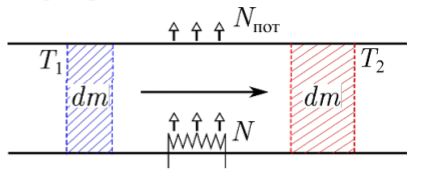
\includegraphics{pic1_211.png}}
\caption{Нагрев газа при течении по трубе}

\end{figure}
		
		
Рассмотрим газ, протекающий стационарно слева направо через трубу постоянного сечения, в кото-рой установлен нагревательный элемент (см.рис.1). Пусть за некоторое время $dt$ через калориметр прошла малая порция газа массой $dm = q dt$ , где $q$ [кг/с] - массовый расход газа в трубе. Если мощность нагрева равна $N$, мощность тепловых потерь на обмен с окружающей средой $N_{\text{пот}}$, то порция получила тепло $\delta Q =(N - N_{\text{пот}})dt$. С другой стороны, по определению теплоёмкости (1): $\delta Q =c dm \Delta T$ , где $\Delta T = T_2 - T_1$ - приращение температуры газа, и $c$ — удельная (на единицу массы) теплоёмкость газа в рассматриваемом процессе. При малых расходах газа и достаточно большом диаметре трубы перепад давления на её концах мал, поэтому можно принять, что $P_1 \approx P_2 = P_0$, где $P_0$ - атмосферное давление. Следовательно, в условиях опыта измеряется удельная теплоёмкость при постоянном давлении $c_P$. Таким образом, получаем

\begin{equation}
C_p = \dfrac{N - N_{\text{пот}}}{q \Delta T} 
\end{equation}

\section{Экспериментальная установка}
 
 Схема установки изображена на рис. 2. Воздух, нагнетаемый компрессором, прокачивается через калориметр. Калориметр представляет собой стеклянную цилиндрическую трубку с двойными стенками, запаянными с торцов.
	
		\begin{figure}[h!]
		\center{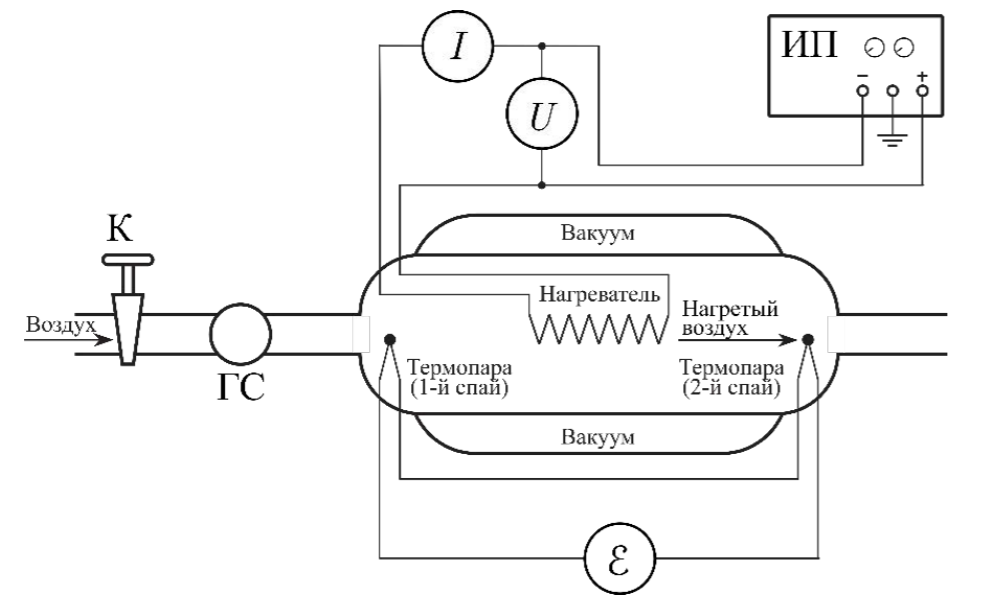
\includegraphics{ust211.png}}
		\end{figure}
	
		Нагреватель в виде намотанной на пенопласт нихромовой проволоки расположен внутри калориметра непосредственно в воздушном потоке. Нагрев проволоки производится от регулируемого источника постоянного тока (ИП).
		Напряжение $U$ на нагревателе и ток $I$ через него регистрируются цифровыми мультиметрами. Таким образом, мощность нагрева равна
		
		\begin{equation}
		    N= UI
		\end{equation}
		Для измерения разности температур $\Delta T$ служит медно-константановая
		термопара. Один спай термопары расположен в струе воздуха, входящего в
		калориметр, и находится при комнатной температуре, а второй — в струе выходящего нагретого воздуха. Константановая проволока термопары расположена внутри калориметра, а медные проводники подключены к цифровому вольтметру. Возникающая в термопаре ЭДС $\varepsilon$ пропорциональна разности температур $\Delta T$ спаев: 
		
		\begin{equation}
		    \varepsilon =\beta \Delta T
		\end{equation}
		
		 где $\beta = 40.7 \frac{мкВ}{^\circ C}$ — чувствительность медно-константановой термопары в рабочем диапазоне температур (20–30$^\circ C$ ). ЭДС регистрируется с помощью микровольтметра.
		
		Объём воздуха, прошедшего через калориметр, измеряется газовым счётчиком ГС. Для регулировки расхода служит кран К. Время $\Delta t$ прохождения
		некоторого объема $\Delta V$ воздуха измеряется секундомером. Объёмный расход равен $\frac{\Delta V}{\Delta t} $, массовый расход может быть найден как 
		
		\begin{equation}
		    q = \rho_{0} \frac{\Delta V}{\Delta t}
		\end{equation}
		
	 где $rho_{0}$ — плотность воздуха при комнатной температуре, которая в свою очередь может быть получена из уравнения Менделеева–Клапейрона: $\rho_{0}= \frac{\mu P_{0} }{R T_{0}},$ где $P_{0}$ — атмосферное давление, $T_{0}$ — комнатная температура (в Кельвинах), $\mu = 29,0 {г/моль}$ — средняя молярная масса (сухого) воздуха.
		
		Учитывая особенности устройства калориметра, следует ожидать, что мощность нагревателя расходуется не только на нагрев массы прокачиваемого воздуха, но и частично теряется за счет нагрева внутренних стенок термостата и рассеяния тепла через торцы термостата. Можно предположить, что при небольшом нагреве ($\Delta T \ll T_{0}$) мощность потерь тепла $N_{пот}$ прямо пропорциональна разности температур:
		\begin{equation}
		    N_{пот} = \alpha \Delta T
		\end{equation}
		
		 где $\alpha$ — некоторая константа. При этом условии основное соотношение (2) принимает вид 
		 \begin{equation}
		    N = (c_{P}q +\alpha)\Delta T
		\end{equation}
		 
		Следовательно, при фиксированном расходе воздуха ($q = const$) подводимая мощность и разность температур связаны прямой пропорциональностью($\Delta T(N)$ — линейная функция).
 
\section{Обработка результатов измерений}


\section{Вывод}


\end{document}
